\documentclass[12pt]{article}
\usepackage[margin=2.5cm]{geometry}
\usepackage[colorlinks=true, linkcolor=blue, urlcolor=blue, citecolor=blue]{hyperref}
\usepackage{tikz}
\usepackage{amsmath}
\usepackage{mathtools}
\usepackage{graphicx}
\setlength{\parindent}{0pt}
\setlength{\parskip}{0.75em}
\usepackage{pgfplots}
\pgfplotsset{compat=1.18}


\title{Chapter 4: Small Oscillations}
\author{İskender Yalçınkaya, PhD}
\date{\today}

\begin{document}
\maketitle
In this chapter, we will study how physical systems behave in the vicinity of their stable equilibrium points. Such behavior is often referred to as \textit{small oscillations} because the system exhibits oscillatory motion about its equilibrium position, with a displacement that remains small.

We will first examine the simplest case of oscillatory motion, in which a restoring force acts on the system, pushing it back toward its equilibrium position. We will then consider the effects of a retarding force, which dissipates mechanical energy and causes the amplitude of oscillations to decrease over time. Finally, we will study driven oscillations, in which an external periodic force acts on the system, and investigate how the resulting motion depends on the frequency of the driving force, including the phenomenon of resonance. For simplicity, we will restrict our attention to one-dimensional systems throughout this chapter.

\section{Simple Oscillations}

We begin by considering the motion of a particle under a conservative force described by a potential energy function $U(x)$. We make the following three assumptions:
\begin{enumerate}
    \item[(i)] $U(x)$ is sufficiently smooth to allow a Taylor expansion about the equilibrium point.
    \item[(ii)] The potential has a local minimum at $x=x_0$, with $U'(x_0)=0$ and $U''(x_0)>0$, so that $x_0$ is a stable equilibrium point.
    \item[(iii)] The displacement from equilibrium, $|x-x_0|$, remains ``sufficiently small''.
\end{enumerate}

Assumption (i) allows us to expand the potential energy about the equilibrium point $x_0$ using a Taylor series:
\begin{equation}
    U(x) = U(x_0) + U'(x_0)(x-x_0)
    + \frac{1}{2}U''(x_0)(x-x_0)^2
    + \frac{1}{6}U'''(x_0)(x-x_0)^3
    + \ldots
\end{equation}
According to assumption (ii), the first derivative vanishes at equilibrium, $U'(x_0)=0$, while the second derivative is positive, $U''(x_0)>0$. Furthermore, assumption (iii) allows us to neglect the third and higher-order terms compared to the quadratic term. This is what we actually mean when we say that the displacement is ``sufficiently small'' in assumption (iii). Since the reference level of potential energy can be chosen arbitrarily, we may also set $U(x_0)=0$ without loss of generality. We therefore obtain the quadratic approximation
\begin{equation}
    U(x) \approx \frac{1}{2}k(x-x_0)^2,
    \label{eq:quadratic-potential}
\end{equation}
where $k\equiv U''(x_0)>0$. It is worth emphasizing that the approximation for the potential energy follows directly from our assumptions and is not limited to specific systems such as springs or pendulums. A wide range of physical systems can be described by a quadratic potential near their stable equilibrium points, provided that the second derivative of the potential at equilibrium is positive. This allows us to study the small oscillations of different physical systems using the same mathematical framework.

\begin{figure}[htbp]
    \centering
    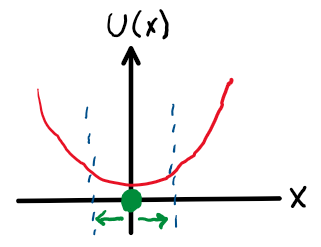
\includegraphics[width=0.4\textwidth]{figures/small-oscillation.png}
    \caption{Small oscillations of a particle about a stable equilibrium point under potential energy $U(x)$. The particle oscillates about the equilibrium position $x_0$ with a small amplitude.}
    \label{fig:small-oscillations}
\end{figure}

Using the quadratic approximation, we can derive the force acting on the particle:
\begin{equation}
    F(x)=-\frac{dU}{dx}\approx -k(x-x_0).
\end{equation}
This is known as \textit{Hooke's law}. The force is proportional to the displacement from equilibrium and always points toward the equilibrium position $x_0$. For this reason, it is called a \textit{restoring force}. The constant $k$ is called the \textit{force constant} or \textit{spring constant}, and it characterizes the stiffness of the system. A larger value of $k$ corresponds to a stiffer system, which requires more force to achieve the same displacement from equilibrium. 

From the experimental point of view, the force constant can be determined by measuring the force required to displace the particle from its equilibrium position and calculating the slope of the force-displacement curve as shown in Fig.~\ref{fig:empirical-force-constant}. The force constant is a fundamental property of the system and depends on its physical characteristics, such as the material properties and geometry.

\begin{figure}[!h]
    \centering
    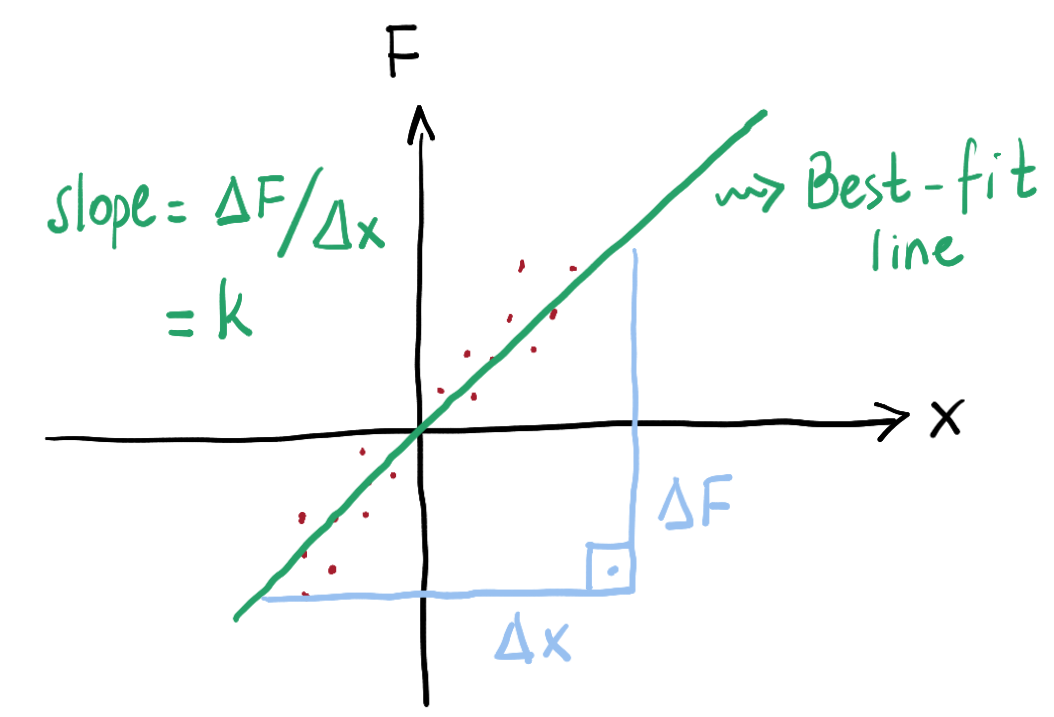
\includegraphics[width=0.58\textwidth]{figures/empirical-force-constant.png}
    \caption{Empirical determination of the force constant $k$. The slope of the force-displacement curve gives the value of $k$. Note that the linear best-fit line is a model; the idea is there is always a sufficiently small region around the equilibrium point where the force is linear in the displacement. The data points may scatter according to different models as the displacement increaases.}
    \label{fig:empirical-force-constant}
\end{figure}

\subsection{Equation of Motion for Simple Oscillations}

The dynamics of the particle are governed by Newton's second law:
\begin{equation}
    F_\text{net}=m\ddot{x},
\end{equation}
where $m$ is the mass of the particle. Assuming that the restoring force is the only net force acting on the particle, and choosing the origin at the equilibrium position ($x_0=0$), we obtain
\begin{equation}
    m\ddot{x}=-kx.
\end{equation}
Rearranging this equation gives
\begin{equation}
    \ddot{x}+\omega_0^2 x=0,
    \label{eq:simple-osc-eq-of-motion}
\end{equation}
where we have introduced the positive parameter
\begin{equation}
    \omega_0\coloneqq\sqrt{\frac{k}{m}}.
    \label{eq:natural-angular-frequency}
\end{equation}

This is a second-order linear homogeneous differential equation describing \textit{simple harmonic motion}. The physical meaning of $\omega_0$ will become clear when we solve this equation and examine the resulting motion.



\subsection{\label{sec:solution-simple-osc}Solution to the Equation of Motion}
We know that the particle oscillates back and forth about the equilibrium position in a periodic way. We saw in Chapter 1 that the exponential function $e^{\lambda t}$ exhibits a wide range of different types of behavior depending on how the parameter $\lambda$ is chosen as summarized in the following table:

\begin{table}[h]
    \centering
    \begin{tabular}{ll}
        \hline
        $\lambda$ & Behavior of $e^{\lambda t}$ \\
        \hline
        Real and positive ($\lambda > 0$) & Exponential growth \\
        Real and negative ($\lambda < 0$) & Exponential decay \\
        Purely imaginary ($\lambda = i$) & Sinusoidal oscillation \\
        Complex, $\operatorname{Re}(\lambda) < 0$ & Oscillation with exponentially decaying amplitude \\
        Complex, $\operatorname{Re}(\lambda) > 0$ & Oscillation with exponentially growing amplitude \\
        \hline
    \end{tabular}
\end{table}

We know that the solution to the differential equation in Eq.~\ref{eq:simple-osc-eq-of-motion} must be oscillatory according to our assumptions. Therefore, it is natural\footnote{I admit that this is a handwaving argument. For the complete description, we need to study Laplace transforms which is beyond the scope of this text.} to look for a solution of the form $x(t)=e^{\lambda t}$, where $\lambda$ will be determined by substituting this ansatz into the differential equation. Differentiating this ansatz twice and pluging it into the equation of motion as given by Eq.~\ref{eq:simple-osc-eq-of-motion} gives
\begin{equation}
    \lambda^2 e^{\lambda t}+ \omega_0^2 e^{\lambda t} = 0 \implies \lambda^2 + \omega_0^2 = 0.
\end{equation}
This equation is called the characteristic equation having the two purely imaginary roots
\begin{equation}
    \lambda_{1,2}=\pm i\omega_0.
\end{equation}
This leads to two different solutions
$x_{1,2}(t)=e^{\pm i\omega_0 t}$. Not surprisingly, the both solutions have a pure complex factor of the time leading to oscillatory behavior.

A second-order linear homogeneous differential equation requires two initial conditions to determine a unique solution; therefore, the linear combination of two linearly independent solutions, containing two arbitrary constants, is sufficient to describe all possible solutions \footnote{The details about the construction of the general solution is a topic of linear algebra and again beyond the scope of this text.}. Thus, the general solution can be written as
\begin{equation}
    x(t)=Ae^{i\omega_0 t}+Be^{-i\omega_0 t},
\end{equation}
where $A$ and $B$ are arbitrary constants determined by the initial conditions. In general, these constants can be complex. However, since $x(t)$ represents the position of a particle, it must be a real-valued function. To express the solution in a real form, we use Euler's formula,
\begin{equation}
    e^{i\theta}=\cos\theta+i\sin\theta,
\end{equation}
which also implies
\begin{equation}
    e^{-i\theta}=\cos\theta-i\sin\theta.
\end{equation}
Substituting these expressions into the general solution gives
\begin{align}
    x(t)
    &=A\left[\cos(\omega_0 t)+i\sin(\omega_0 t)\right]
    +B\left[\cos(\omega_0 t)-i\sin(\omega_0 t)\right]
    \nonumber\\
    &=(A+B)\cos(\omega_0 t)
    +i(A-B)\sin(\omega_0 t).
\end{align}

At first glance, the coefficients $A+B$ and $i(A-B)$ may appear to be complex. However, we can show that they must be real by considering the initial conditions. Suppose that the particle has an initial position $x(0)=x_0$ and an initial velocity $\dot{x}(0)=v_0$. Evaluating the position at $t=0$, we obtain
\begin{equation}
    x(0)=A+B=x_0.
\end{equation}
Differentiating the solution with respect to time gives
\begin{equation}
    \dot{x}(t)
    =-\omega_0(A+B)\sin(\omega_0 t)
    +i\omega_0(A-B)\cos(\omega_0 t).
\end{equation}
Evaluating the velocity at $t=0$, we find
\begin{equation}
    \dot{x}(0)=i\omega_0(A-B)=v_0,
\end{equation}
and therefore
\begin{equation}
    A+B=x_0,
    \qquad
    i(A-B)=\frac{v_0}{\omega_0}.
\end{equation}

Since both the initial position $x_0$ and the initial velocity $v_0$ are real physical quantities, the combinations $A+B$ and $i(A-B)$ must also be real. Substituting these expressions back into the general solution, we finally obtain
\begin{equation}
    x(t)=x_0\cos(\omega_0 t)
    +\frac{v_0}{\omega_0}\sin(\omega_0 t).
\end{equation}

This expression describes the motion of the particle
for any given initial position $x_0$ and initial
velocity $v_0$. For convenience, we can introduce two real constants,
$C=x_0$ and $D=v_0/\omega_0$, and write the general
solution in the more compact form
\begin{equation}
    x(t)=C\cos(\omega_0 t)+D\sin(\omega_0 t).
    \label{eq:general-solution}
\end{equation}
The constants $C$ and $D$ are determined by the initial conditions. 

\subsection{Amplitude-Phase Form of the General Solution}

This general solution given in Eq.~\ref{eq:general-solution} can also be expressed in terms of the \emph{amplitude} and \emph{phase} of the oscillation. To see this, we start from Eq.~\ref{eq:general-solution} and use Euler's formula to rewrite the trigonometric functions in terms of complex exponentials:
\begin{align}
    x(t)
    &=C\operatorname{Re}\left[e^{i\omega_0 t}\right]+D\operatorname{Re}\left[-i e^{i\omega_0 t}\right]\nonumber\\
    &=\operatorname{Re}\left[
    Ce^{i\omega_0 t}-iDe^{i\omega_0 t}
    \right]\nonumber\\
    &=\operatorname{Re}\left[
    (C-iD)e^{i\omega_0 t}
    \right],
\end{align}
where $\operatorname{Re}$ denotes the real part of a complex number. We now introduce the complex number
\begin{equation}
    Z\coloneqq C-iD,
\end{equation}
which is constant and called a \emph{phasor} or \emph{complex amplitude}. Recall that any nonzero complex number can be expressed in polar form as $Z=Re^{i\phi}$, where $R=|Z|$ is its magnitude and $\phi$ is its argument. Since $Z=C-iD$, its magnitude and argument can be determined from the real and imaginary parts:
\begin{equation}
    R=\sqrt{C^2+D^2},\qquad 
    \phi=\arctan\left(-\frac{D}{C}\right).
\end{equation}

Substituting the polar form of $Z$ into the expression for the displacement gives
\begin{align}
    x(t)
    &=\operatorname{Re}\left[Ze^{i\omega_0 t}\right]
    \nonumber\\
    &=\operatorname{Re}\left[Re^{i\phi}e^{i\omega_0 t}\right]
    \nonumber\\
    &=\operatorname{Re}\left[Re^{i(\omega_0 t+\phi)}\right].
\end{align}
Finally, using Euler's formula, we obtain
\begin{equation}
    x(t)=R\cos(\omega_0 t+\phi).
    \label{eq:amplitude-phase-form}
\end{equation}
This is called the \emph{amplitude-phase form} of the general solution.  Recalling that $C=x_0$ and $D=v_0/\omega_0$, the amplitude and the initial phase can be expressed in terms of the initial conditions as
\begin{equation}
    R=\sqrt{x_0^2+\frac{v_0^2}{\omega_0^2}},\qquad 
    \phi=\arctan\left(-\frac{v_0}{\omega_0 x_0}\right).
    \label{eq:amplitude-phase-initial-conditions}
\end{equation}
The phasor representation also provides a geometric interpretation of the motion as shown in Fig.~\ref{fig:phasor-representation}. The complex quantity $Re^{i(\omega_0 t+\phi)}$ represents a vector of constant length $R$ rotating counterclockwise in the complex plane with angular velocity $\omega_0$. The projection of this rotating vector onto the real axis gives the physical displacement $x(t)$ of the particle.

\begin{figure}[!htbp]
    \centering
    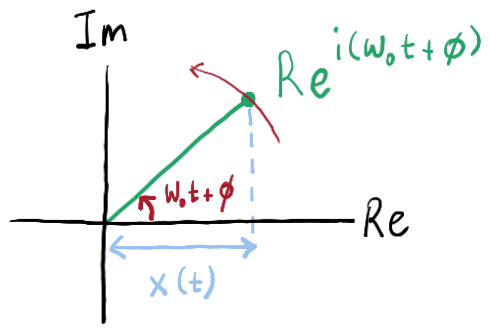
\includegraphics[width=0.45\textwidth]{figures/phasor-representation.png}
    \caption{Phasor representation of simple harmonic motion. The complex vector $Re^{i(\omega_0 t+\phi)}$ rotates in the complex plane, and its projection onto the real axis gives the physical displacement $x(t)$.}
    \label{fig:phasor-representation}
\end{figure}

\subsection{Physical Interpretation of the General Solution}

In the general solution given in Eq.~\eqref{eq:amplitude-phase-form}, the constant $R\geq 0$ is called the \emph{amplitude}, representing the maximum displacement of the particle from its equilibrium position. The constant $\phi$ is called the \emph{initial phase} (or \emph{phase constant}), which determines where in its oscillation cycle the particle is at $t=0$. In other words, the initial phase determines at what point in the oscillation we start our chronometer. The constant $\omega_0$ is the \emph{angular frequency}, which determines how rapidly the particle oscillates. Recall from Eq.~\eqref{eq:natural-angular-frequency} that $\omega_0=\sqrt{k/m}$, where $k$ is the force constant and $m$ is the mass of the particle. Thus, a stiffer system (larger $k$) or a lighter particle (smaller $m$) oscillates more rapidly. In Fig.~\ref{fig:general-solution}, you can see how $x(t)$ varies with time.

The motion is \emph{periodic}, meaning that both the position and velocity of the particle repeat after a fixed time interval called the \emph{period} $T$. For simple harmonic motion, the period is
\begin{equation}
    T=\frac{2\pi}{\omega_0}.
\end{equation}
The \emph{frequency} $f$ is the number of complete oscillations
per unit time and is given by
\begin{equation}
    f=\frac{1}{T}=\frac{\omega_0}{2\pi}.
\end{equation}
The frequency is measured in hertz (Hz), while the angular frequency is measured in radians per second (rad/s).

As shown in Eq.~\eqref{eq:amplitude-phase-initial-conditions}, both the amplitude $R$ and the initial phase $\phi$ are determined by the initial position and velocity of the particle. Unlike these two quantities, the angular frequency $\omega_0$ depends only on the physical properties of the oscillator and not on its initial conditions. Consequently, the period of simple harmonic motion is independent of the amplitude of oscillation.

Finally, in the special case $R=0$, the particle remains at its equilibrium position, $x(t)=0$, and the phase $\phi$ is undefined.

\begin{figure}[!htbp]
    \centering
    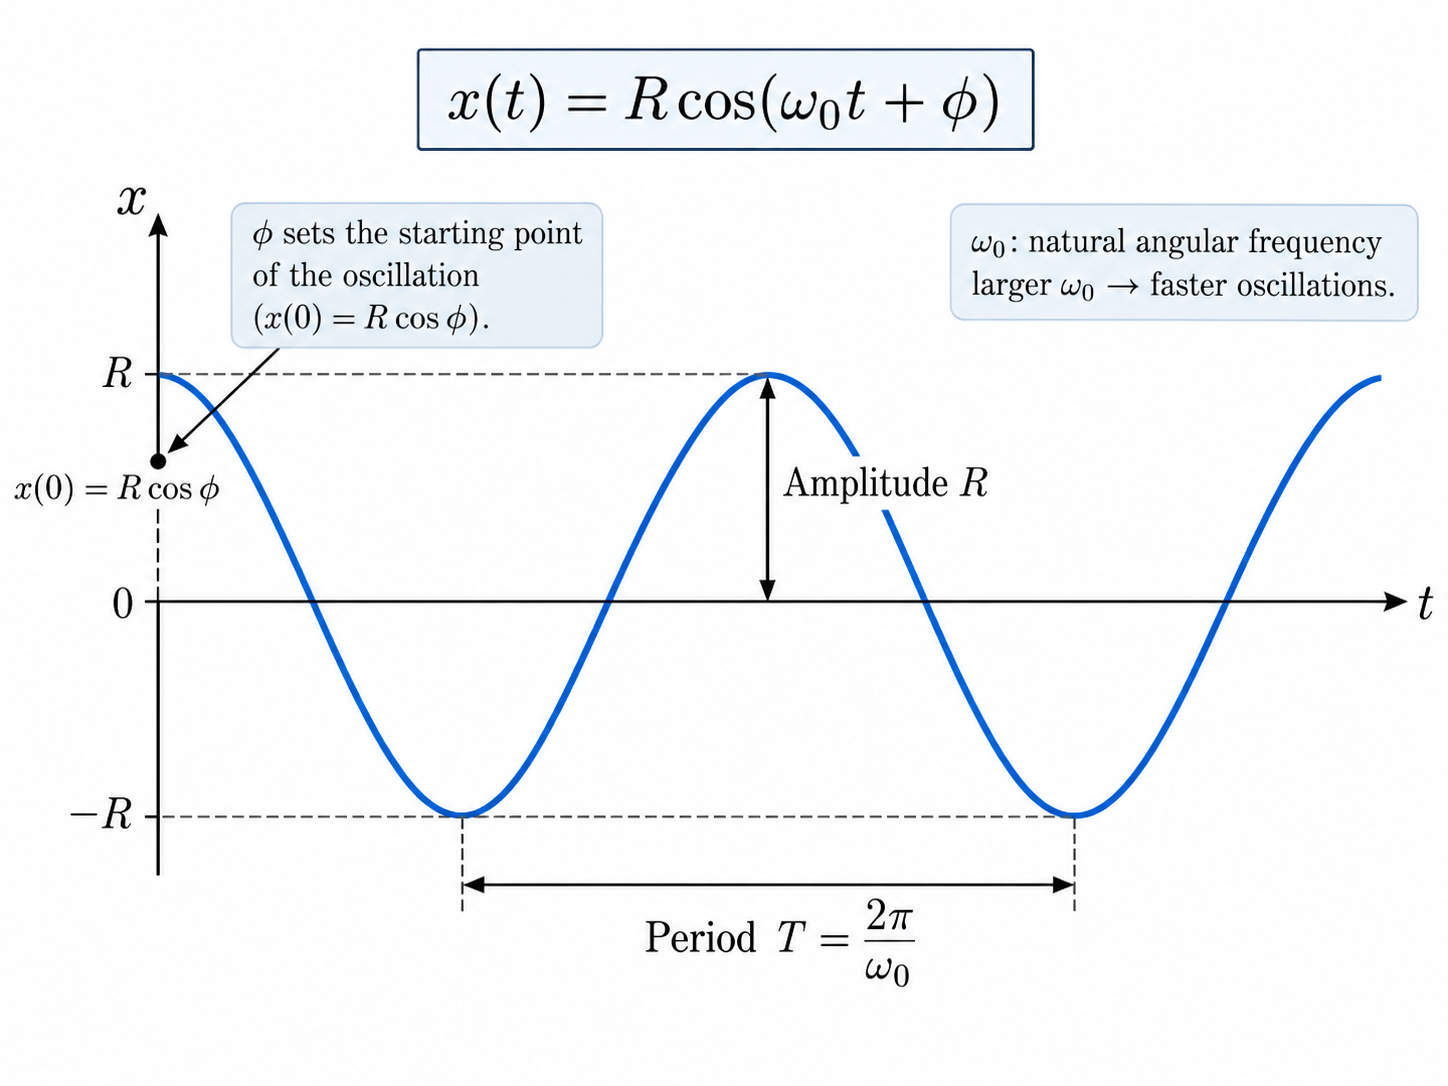
\includegraphics[width=0.6\textwidth]{figures/general-solution.png}
    \caption{General solution of simple harmonic motion. The particle oscillates about the equilibrium position with amplitude $R$ and angular frequency $\omega_0$. The initial phase $\phi$ determines the starting point of the oscillation at $t=0$.}
    \label{fig:general-solution}
\end{figure}

\subsection{Energy of Simple Oscillations}
The mechanical energy of a particle undergoing simple oscillation
\begin{equation}
    E = K + U = \frac{1}{2} m \dot{x}^2 + \frac{1}{2} k x^2 
\end{equation}

Substituting the general solution $x(t)=R\cos(\omega_0 t+\phi)$ into the expressions for kinetic and potential energies, we find
\begin{align}
    K(t)&=\frac{1}{2}m\left[-R\omega_0\sin(\omega_0 t+\phi)\right]^2
    =\frac{1}{2}mR^2\omega_0^2\sin^2(\omega_0 t+\phi),\\
    U(t)&=\frac{1}{2}k\left[R\cos(\omega_0 t+\phi)\right]^2
    =\frac{1}{2}kR^2\cos^2(\omega_0 t+\phi).
\end{align}
Using the relation $k=m\omega_0^2$, we can express the total energy as
\begin{equation}
    E=\frac{1}{2}mR^2\omega_0^2\left[\sin^2(\omega_0 t+\phi)+\cos^2(\omega_0 t+\phi)\right]
    =\frac{1}{2}mR^2\omega_0^2.
\end{equation}
By substituting $\omega_0^2=k/m$, we can also express the total energy in terms of the force constant $k$ and the amplitude $R$:
\begin{equation}
    E=\frac{1}{2}kR^2.
\end{equation}
Hence, the mechanical energy of a simple oscillator is constant and proportional to the square of the amplitude. This is a characteristic feature of conservative systems, where energy is conserved and oscillates between kinetic and potential forms without any loss as shown in the Fig.~\ref{fig:energy-oscillations}, with the maximum kinetic energy occurring when the particle passes through the equilibrium position ($x=0$) and the maximum potential energy occurring at the turning points of the motion ($x=\pm R$).

\begin{figure}[!h]
    \centering
    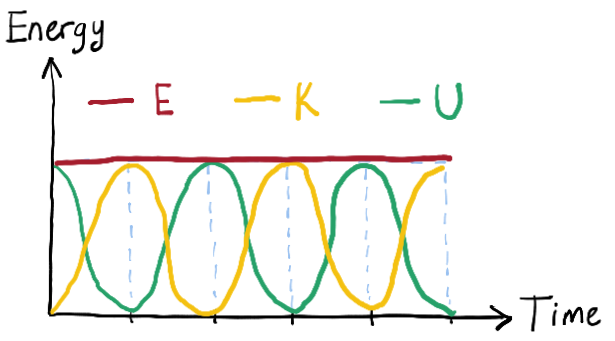
\includegraphics[width=0.6\textwidth]{figures/energy-oscillations.png}
    \caption{Oscillations of kinetic energy $K(t)$, potential energy $U(t)$, and total energy $E$ for a particle undergoing simple harmonic motion. The total energy remains constant, while the kinetic and potential energies oscillate out of phase with each other.}
    \label{fig:energy-oscillations}
\end{figure}


\section{Damped Oscillations}  
If the oscillating system is not isolated, it may experience a retarding force that dissipates mechanical energy. We will consider a model in which the retarding force is proportional to the velocity of the particle, which is a common situation in many physical systems. The retarding force can be expressed as
\begin{equation}
    F_\text{r}=-b\dot{x},
\end{equation}
where $b$ is a positive constant called the \textit{damping coefficient}. The negative sign indicates that the retarding force opposes the motion of the particle. The damping coefficient has units of force per unit velocity (N·s/m) and depends on the properties of the medium through which the particle moves, such as viscosity or air resistance. The total force acting on the particle is then the sum of the restoring force and the retarding force:
\begin{equation}
    F_\text{net}=F_\text{restoring}+F_\text{retarding}=-kx-b\dot{x}.
\end{equation}

This leads to the equation of motion for damped oscillations:
\begin{equation}
    m\ddot{x}+b\dot{x}+kx=0.
\end{equation}
Rearranging this equation gives
\begin{equation}
    \ddot{x}+2\gamma\dot{x}+\omega_0^2 x=0,
    \label{eq:damped-osc-eq-of-motion}
\end{equation}
where we have introduced the positive parameters
\begin{equation}
    \gamma\coloneqq \frac{b}{2m},
    \qquad
    \omega_0\coloneqq \sqrt{\frac{k}{m}}.
\end{equation}

We would expect that the damping force would cause the amplitude of oscillations to decrease over time, eventually bringing the particle to rest at its equilibrium position. The parameter $\gamma$ characterizes the strength of the damping, with larger values corresponding to stronger damping effects. The parameter $\omega_0$ is the natural angular frequency of the undamped system, as we have seen in the previous section.

We know that the exponential function $e^{\lambda t}$ exhibits a wide range of different types of behavior depending on how the parameter $\lambda$ is chosen. For the damped oscillation equation, we can look for a solution of the form $x(t)=e^{\lambda t}$, as we did it in Section \ref{sec:solution-simple-osc} for simple oscillations. Plugging this into the differential equation in Eq.~\ref{eq:damped-osc-eq-of-motion} leads to the characteristic equation
\begin{equation}
    \lambda^2+2\gamma\lambda+\omega_0^2=0,
\end{equation}
which has the two roots
\begin{equation}
    \lambda_{1,2}=\frac{-2\gamma\pm\sqrt{(2\gamma)^2-4\omega_0^2}}{2}=-\gamma\pm\sqrt{\gamma^2-\omega_0^2}.
\end{equation}
The roots can be real or complex, depending on the relative magnitudes of $\gamma$ and $\omega_0$, leading to three different cases: underdamped ($\gamma<\omega_0$), critically damped ($\gamma=\omega_0$), and overdamped ($\gamma>\omega_0$). Each case corresponds to a different type of motion, which we will analyze in detail in the following subsections.

\subsection{Underdamped Oscillations ($\gamma<\omega_0$)}
In the underdamped case, the damping is weak enough that the system still oscillates, but with a gradually decreasing amplitude. The roots of the characteristic equation are complex conjugates:
\begin{equation}
    \lambda_{1,2}=-\gamma\pm i\omega_1,
\end{equation}
where we have defined the \textit{damped angular frequency}
\begin{equation}
    \omega_1\coloneqq\sqrt{\omega_0^2-\gamma^2}.
\end{equation}
The solution to the differential equation in this case is
\begin{equation}
    x(t)=e^{-\gamma t}(Ae^{i\omega_1 t}+Be^{-i\omega_1 t}),
    \label{eq:underdamped-solution}
\end{equation}
where $A$ and $B$ are constants determined by the initial conditions. According to Eq.~\ref{eq:amplitude-phase-form}, we can also express the solution in amplitude-phase form as
\begin{equation}
    x(t)=(Re^{-\gamma t})\cos(\omega_1 t+\phi),
    \label{eq:underdamped-amplitude-phase}
\end{equation}
where $R$ is the initial amplitude and $\phi$ is the initial phase. What we see inside the parantheses is the amplitude of the oscillation, which decays exponentially over time due to the damping effect. On the other hand, the cosine term describes the oscillatory motion with angular frequency $\omega_1$. Therefore, the motion is a combination of exponential decay and sinusoidal oscillation as shown in Fig.~\ref{fig:underdamped-oscillations}. 
\begin{figure}[!htbp]
    \centering
    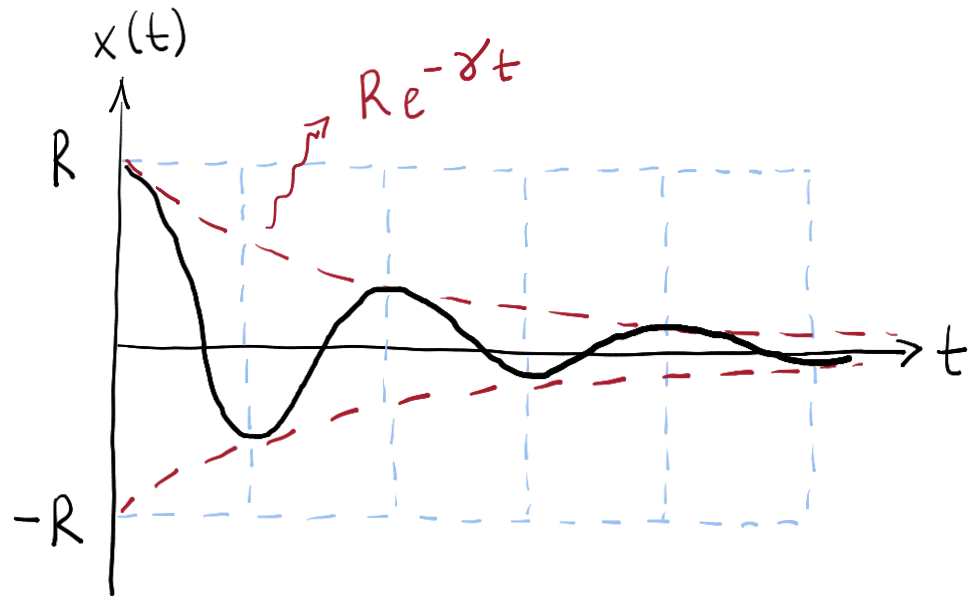
\includegraphics[width=0.65\textwidth]{figures/underdamped-oscillations.png}
    \caption{Underdamped oscillations of a particle. The amplitude of oscillation decays exponentially over time due to the damping effect, while the particle continues to oscillate with a damped angular frequency $\omega_1$.}
    \label{fig:underdamped-oscillations}
\end{figure}


Directly followed from the definition of $\omega_1$, the damped angular frequency $\omega_1$ is slightly less than the natural angular frequency $\omega_0$, indicating that the oscillations occur at a lower frequency than in the undamped case
\[
    \omega_1=\sqrt{\omega_0^2-\gamma^2}<\omega_0.
\]

Strictly speaking, the word ``frequency'' attributed to periodic motion. Therefore, calling $\omega_1$ a frequency is not strictly correct, since the motion is not strictly periodic due to the damping. However, it is common practice to refer to $\omega_1$ as the damped angular frequency, as it characterizes the rate of oscillation in the presence of damping for a given time interval.

We know that the mechanical energy of a simple oscillator is constant and proportional to the square of its amplitude. In the case of underdamped oscillations, the amplitude decreases exponentially over time, resulting in a corresponding loss of mechanical energy. Since both the displacement and velocity acquire
the same exponential factor $e^{-\gamma T}$ after
one complete period $T$, the mechanical energy
satisfies
\begin{equation}
    E(t+T)=E(t)e^{-2\gamma T}.
\end{equation}
Consequently, after $n$ complete periods,
\begin{equation}
    E(nT)=E_0e^{-2\gamma nT},
\end{equation}
where $E_0$ is the initial mechanical energy.
The decrease in mechanical energy is due to
dissipation, typically involving its conversion
into heat or other forms of energy.


\subsection{Critically Damped Oscillations ($\gamma=\omega_0$)}

In the critically damped case, the damping is just strong enough to prevent oscillations. The roots of the characteristic equation are real and equal:
\begin{equation}
    \lambda_{1,2}=-\gamma.
\end{equation}
Therefore, we do not have two distinct solutions. We mentioned in Sec.~\ref{sec:solution-simple-osc} that the general solution for a second-order linear differential equation with constant coefficients is a linear combination of two independent solutions. In this case, we have only one independent solution, which is $e^{-\gamma t}$. To find a second independent solution, we return to the equation of motion, which, for $\gamma=\omega_0$,
takes the form
\begin{equation}
    \ddot{x}+2\gamma\dot{x}+\gamma^2 x=0.
\end{equation}
Multiplying both sides by $e^{\gamma t}$, we obtain
\begin{equation}
    e^{\gamma t}\ddot{x}
    +2\gamma e^{\gamma t}\dot{x}
    +\gamma^2 e^{\gamma t}x=0.
\end{equation}
Note that the left-hand side is precisely the second derivative of the product $e^{\gamma t}x(t)$, as can be verified by applying the product rule twice:
\begin{equation}
    \frac{d^2}{dt^2}\left[e^{\gamma t}x(t)\right]
    =e^{\gamma t}\ddot{x}
    +2\gamma e^{\gamma t}\dot{x}
    +\gamma^2 e^{\gamma t}x.
\end{equation}
Therefore, the equation of motion can be rewritten as
\begin{equation}
    \frac{d^2}{dt^2}\left[e^{\gamma t}x(t)\right]=0.
\end{equation}
Integrating twice with respect to time gives
\begin{equation}
    e^{\gamma t}x(t)=A+Bt,
\end{equation}
where $A$ and $B$ are arbitrary constants. Solving for $x(t)$, we obtain
\begin{equation}
    x(t)=(A+Bt)e^{-\gamma t}.
\end{equation}
We can now identify the two linearly independent solutions:
\begin{equation}
    x_1(t)=e^{-\gamma t},
    \qquad
    x_2(t)=te^{-\gamma t}.
\end{equation}
Indeed, neither solution can be expressed as a constant multiple of the other, so they are linearly independent. The constants $A$ and $B$ can be determined from the initial conditions $x(0)=x_0$ and $\dot{x}(0)=v_0$. Substituting these conditions gives
\begin{equation}
    A=x_0,
    \qquad
    B=v_0+\gamma x_0.
\end{equation}
Thus, the motion of a critically damped oscillator is
described by
\begin{equation}
    x(t)=\left[x_0+(v_0+\gamma x_0)t\right]e^{-\gamma t}.
\end{equation}
Since both $e^{-\gamma t}$ and $te^{-\gamma t}$
approach zero as $t\to\infty$, the particle eventually
returns to its equilibrium position without undergoing
oscillations. Depending on the initial conditions, the
particle may cross the equilibrium position once, but
it cannot oscillate back and forth around it. 
\subsection{Overdamped Motion ($\gamma>\omega_0$)}

In the overdamped case, the damping is sufficiently strong to prevent oscillations. The roots of the characteristic equation are real and distinct:
\begin{equation}
    \lambda_{1,2}=-\gamma\pm\sqrt{\gamma^2-\omega_0^2}.
\end{equation}
Since $\gamma>\omega_0$, both roots are negative,
with $\lambda_2<\lambda_1<0$.
The general solution to the differential equation is
\begin{equation}
    x(t)=Ae^{\lambda_1 t}+Be^{\lambda_2 t},
    \label{eq:overdamped-solution}
\end{equation}
where $A$ and $B$ are constants determined by the initial conditions.

Since both exponential terms decay with time, the particle eventually approaches its equilibrium position. However, the two terms decay at different rates. Since $\lambda_1>\lambda_2$, the term $e^{\lambda_1 t}$ decays more slowly and dominates the motion at sufficiently long times, provided $A\neq 0$.

Unlike the critically damped case, overdamping generally results in a slower approach to equilibrium. Although the particle may cross the equilibrium position once, depending on its initial conditions, it cannot undergo oscillatory
motion about equilibrium.


Since $\lambda_2<\lambda_1<0$, both exponential terms
decay with time. At sufficiently long times, the term
$e^{\lambda_1 t}$ dominates, provided $A\neq 0$.
Notice that
\begin{equation}
    \lambda_1
    =-\frac{\omega_0^2}
    {\gamma+\sqrt{\gamma^2-\omega_0^2}}
    >-\omega_0,
\end{equation}
where we have used $\gamma>\omega_0$.
Thus, the dominant exponential decays more slowly than
the exponential factor $e^{-\omega_0 t}$ appearing in
the critically damped solution. Overdamping therefore
generally produces a slower relaxation toward equilibrium.

Furthermore, the particle can cross equilibrium only when $x(t)=0$, which, for nonzero $A$ and $B$, requires
\begin{equation}
    e^{(\lambda_1-\lambda_2)t}=-\frac{B}{A}.
\end{equation}
Since the left-hand side is a strictly increasing
function of time, this equation can have at most one solution. Consequently, the particle may cross equilibrium once, depending on its initial conditions, but it cannot undergo oscillatory motion.





\subsection{Quality Factor}

The \emph{quality factor} $Q$ is a dimensionless quantity that characterizes how weakly an oscillating system is damped. We know that an undamped oscillator conserves its
mechanical energy, whereas a damped oscillator gradually loses energy. A natural way to characterize the strength of damping is therefore to compare the mechanical energy stored in the oscillator with the energy dissipated during
one complete oscillation.

For weak damping ($\gamma\ll\omega_0$), the quality factor can be expressed approximately as
\begin{equation}
    Q\approx 2\pi\frac{E(t)}{\Delta E},
\end{equation}
where $E(t)$ is the mechanical energy at tan arbitrary time and $\Delta E$ is the energy dissipated over the subsequent oscillation period $T$. The factor $2\pi$ is included by convention. A high quality factor corresponds to weak damping, meaning that the oscillator loses only a small fraction of its mechanical energy during
each cycle. To relate the quality factor to the damping parameter $\gamma$, we recall that the displacement and velocity of an underdamped oscillator is given by
\begin{equation}
    x(t)=R_0 e^{-\gamma t}\cos(\omega_1 t+\phi),
    \qquad
    \dot{x}(t)=-R_0 e^{-\gamma t}\left[\gamma\cos(\omega_1 t+\phi)+\omega_1\sin(\omega_1 t+\phi)\right].
\end{equation}
After one complete oscillation period
$T=2\pi/\omega_1$, the trigonometric functions
return to their original values. Consequently,
both the displacement and velocity are multiplied
by the same exponential factor:
\begin{equation}
    x(t+T)=e^{-\gamma T}x(t),
    \qquad
    v(t+T)=e^{-\gamma T}v(t).
\end{equation}
Since the total mechanical energy is given by $E(t)=\frac12 mv^2(t)+\frac12 kx^2(t)$, we obtain
\begin{align}
    E(t+T)
    &=\frac12 m v^2(t+T)
      +\frac12 k x^2(t+T)\nonumber\\
    &=e^{-2\gamma T}
      \left[\frac12 mv^2(t)
      +\frac12 kx^2(t)\right].
\end{align}
Therefore,
\begin{equation}
    E(t+T)=E(t)e^{-2\gamma T}.
\end{equation}
The mechanical energy dissipated during
one complete oscillation is
\begin{align}
    \Delta E
    &=E(t)-E(t+T)\nonumber\\
    &=E(t)\left(1-e^{-2\gamma T}\right).
\end{align}

For weak damping ($\gamma\ll\omega_0$), we have
$2\gamma T\ll 1$. Using the first-order Taylor
approximation
\begin{equation}
    e^{-2\gamma T}\approx 1-2\gamma T,
\end{equation}
we obtain
\begin{equation}
    \frac{\Delta E}{E(t)}\approx 2\gamma T.
\end{equation}
Substituting this result into the expression for
the quality factor gives
\begin{equation}
    Q\approx\frac{2\pi}{2\gamma T}
    =\frac{\pi}{\gamma T}
    =\frac{\omega_1}{2\gamma}.
\end{equation}
Since $\omega_1=\sqrt{\omega_0^2-\gamma^2}
\approx\omega_0$ for weak damping, we obtain
\begin{equation}
    Q\approx\frac{\omega_0}{2\gamma}.
\end{equation}

For the linearly damped harmonic oscillator, this last expression is conventionally adopted as the exact definition of the quality factor:
\begin{equation}
    Q\coloneqq\frac{\omega_0}{2\gamma}.
    \label{eq:quality-factor}
\end{equation}
Its interpretation in terms of the energy dissipated per oscillation, however, is valid approximately in the weak-damping regime as described above. Rearranging the energy-based expression for the quality factor gives
\begin{equation}
    \frac{\Delta E}{E(t)}
    \approx\frac{2\pi}{Q}.
\end{equation}
This relation provides a direct physical interpretation
of $Q$: the larger the quality factor, the smaller
the fraction of mechanical energy dissipated during
each oscillation. For example, an oscillator with
$Q=100$ loses approximately
\begin{equation}
    \frac{\Delta E}{E(t)}
    \approx\frac{2\pi}{100}\approx 0.063,
\end{equation}
or about $6\%$ of its mechanical energy per cycle.The quality factor also allows us to express the damped angular frequency $\omega_1$ in terms of the natural angular frequency $\omega_0$. Using Eq. \eqref{eq:quality-factor}, we find
\begin{equation}
    \omega_1=\sqrt{\omega_0^2-\gamma^2}
    =\omega_0\sqrt{1-\frac{1}{4Q^2}}.
\end{equation}
For example, when $Q=10$, we obtain $\omega_1\approx0.9987\omega_0$. Thus, for weak damping, the oscillation frequency remains very close to the natural frequency, even though the amplitude gradually decreases with time. Even for $Q=2$, we have $\omega_1\approx0.968\omega_0$, which is still a relatively small deviation from the natural frequency. To obtain another physical interpretation of $Q$, let us determine how many oscillation cycles occur before the amplitude decreases to $1/e$ of its initial value. The amplitude decays according to
\begin{equation}
    R(t)=R_0e^{-\gamma t},
\end{equation}
where $R_0$ is the initial amplitude. The time required for the amplitude to decrease to $R_0/e$ is therefore
\begin{equation}
    t_{1/e}=\frac{1}{\gamma}.
\end{equation}
The number of oscillation cycles during this time is
\begin{equation}
    N=\frac{t_{1/e}}{T}
    =\frac{\omega_1}{2\pi\gamma}.
\end{equation}
For weak damping, $\omega_1\approx\omega_0$, and hence
\begin{equation}
    N\approx\frac{Q}{\pi} \implies Q\approx\pi N.
\end{equation}
This result shows that the quality factor is directly proportional to the number of oscillation cycles required for the amplitude to decrease to $1/e$ of its initial value. For example, an oscillator with $Q=100$ completes approximately $32$ cycles during this time. Thus, the quality factor provides two complementary physical interpretations of damping: it characterizes both the fraction of mechanical energy dissipated during each oscillation cycle and the number of cycles over which the oscillation amplitude significantly decreases.



\section{Phase Space and Phase Trajectories}

The \emph{state} of a particle undergoing one-dimensional oscillatory motion is completely specified at any instant by its position $x(t)$ and velocity $\dot{x}(t)$. These quantities can be regarded as coordinates in a two-dimensional space called \emph{phase space}, with position along the horizontal axis and velocity along the vertical axis. The state of the particle is then represented by a point in phase space, and as time progresses, this point traces out a curve called a \emph{phase trajectory}. To determine the phase trajectory of a simple harmonic oscillator, we eliminate time from the equations for position and velocity:
\begin{align}
    x(t) &= R\cos(\omega_0 t+\phi),\\
    \dot{x}(t) &= -R\omega_0\sin(\omega_0 t+\phi).
\end{align}
Squaring both equations, adding them, and using the identity
$\sin^2\theta+\cos^2\theta=1$, we obtain
\begin{equation}
    \frac{x^2}{R^2}
    +\frac{\dot{x}^2}{R^2\omega_0^2}=1.
\end{equation}
This is the equation of an ellipse in phase space, with semi-axes $R$ and $R\omega_0$. Recall that the total mechanical energy of a simple harmonic oscillator is conserved and can be expressed in terms of its amplitude as
\begin{equation}
    E=\frac{1}{2}kR^2
    =\frac{1}{2}m\omega_0^2R^2.
\end{equation}
Substituting this expression into the equation of
the ellipse gives
\begin{equation}
    \frac{x^2}{2E/k}
    +\frac{\dot{x}^2}{2E/m}=1.
\end{equation}
Thus, the phase trajectories form a family of ellipses, each corresponding to a different value of the conserved mechanical energy $E$. As the particle oscillates, its state moves clockwise along the corresponding ellipse, completing one revolution during each oscillation period.

\subsection{Description of Time Evolution in Phase Space}
Let us denote the state of the particle at time $t$ by the vector
\begin{equation}
    \mathbf{X}(t)=\begin{bmatrix}x(t)\\\dot{x}(t)\end{bmatrix}.
\end{equation}
Note that this vector lives in the abstract phase space, which is a two-dimensional space with coordinates $(x, \dot{x})$. It does not correspond to a point in physical space. However, it is still a vector in the sense that it has both magnitude and direction. For example, if we consider the time rate of change of this vector, we consider the time rate of change of the each component. Thus, we get the velocity of the particle in phase space,
\begin{equation}
    \frac{d\mathbf{X}}{dt}=\begin{bmatrix}\dot{x}(t)\\\ddot{x}(t)\end{bmatrix}.
\end{equation}
where the first component is the velocity and the second component is the acceleration of the particle. The second component is defined by Newton's second law. The time evolution of the state vector is governed by the equation
\begin{equation}
    \frac{d\mathbf{X}}{dt}=\begin{bmatrix}\dot{x}(t)\\\ddot{x}(t)\end{bmatrix}
    =\begin{bmatrix}\dot{x}(t)\\-\omega_0^2 x(t)\end{bmatrix}
    =\begin{bmatrix}0&1\\-\omega_0^2&0\end{bmatrix}\mathbf{X}(t).
\end{equation}
This is a first-order linear differential equation for the state vector $\mathbf{X}(t)$, which can be solved using standard techniques. The solution describes how the state of the particle evolves in phase space over time. The matrix
\begin{equation}
    \mathbf{A}=\begin{pmatrix}0&1\\-\omega_0^2&0\end{pmatrix}
\end{equation}
is called the \emph{system matrix}, and its eigenvalues determine the stability and nature of the motion. For a simple harmonic oscillator, the eigenvalues are purely imaginary, indicating that the motion is stable and oscillatory. The corresponding eigenvectors define the directions in phase space along which the state vector evolves. The phase trajectories are closed curves, reflecting the periodic nature of the motion.




\section{Driven Oscillations}


\section{Worked Examples}
\subsection{Work done by the spring force}
\subsection{Simple pendulum}

\subsection{Crossing the Equilibrium Position in Critically Damped Motion}

Consider a critically damped oscillator with damping constant
$\gamma=1\,\mathrm{s}^{-1}$. Initially, the particle is at
$x_0=1\,\mathrm{m}$ and has velocity $v_0=-2\,\mathrm{m/s}$.

\begin{enumerate}
    \item[(a)] Determine the position of the particle as a function of time.
    \item[(b)] Find the time at which the particle crosses the equilibrium position.
    \item[(c)] Determine the maximum displacement of the particle on the opposite side of equilibrium and explain why the motion is not oscillatory.
\end{enumerate}

\textbf{Solution:}

(a) The general solution for critically damped motion is
\begin{equation}
    x(t)=\left[x_0+(v_0+\gamma x_0)t\right]e^{-\gamma t}.
\end{equation}
Substituting the given initial conditions, we obtain
\begin{equation}
    \boxed{x(t)=(1-t)e^{-t},}
\end{equation}
where $t$ is measured in seconds and $x$ in meters.

(b) The particle crosses the equilibrium position when $x(t)=0$.
Therefore,
\begin{equation}
    (1-t)e^{-t}=0.
\end{equation}
Since the exponential function never vanishes, we must have
\begin{equation}
    1-t=0.
\end{equation}
Thus, the particle crosses the equilibrium position at
\begin{equation}
    \boxed{t=1\,\mathrm{s}.}
\end{equation}

(c) To determine the maximum displacement on the opposite side
of equilibrium, we find when the velocity vanishes.
Differentiating the position with respect to time gives
\begin{equation}
    v(t)=\dot{x}(t)=(t-2)e^{-t}.
\end{equation}
Setting $v(t)=0$, we obtain
\begin{equation}
    (t-2)e^{-t}=0,
\end{equation}
which gives
\begin{equation}
    t=2\,\mathrm{s}.
\end{equation}
Substituting this into the position function, we find
\begin{equation}
    x(2)=(1-2)e^{-2}=-e^{-2}\,\mathrm{m}.
\end{equation}
Therefore, the particle reaches its maximum displacement
on the opposite side of equilibrium at
\begin{equation}
    \boxed{x_{\min}=-e^{-2}\,\mathrm{m}\approx-0.135\,\mathrm{m}.}
\end{equation}

The particle initially moves toward equilibrium, crosses it
at $t=1\,\mathrm{s}$, and continues into the negative region.
At $t=2\,\mathrm{s}$, it momentarily stops and reverses direction,
approaching equilibrium from below as $t\to\infty$.

Although the particle crosses the equilibrium position once,
the motion is not oscillatory because it never crosses
equilibrium again. This illustrates that critical damping
does not necessarily prevent a particle from crossing
equilibrium; rather, it prevents repeated oscillations
about equilibrium.

\end{document}
